\documentclass[conference]{IEEEtran}

\usepackage{array}
\usepackage{booktabs}
\usepackage{graphicx}
\usepackage{url}
\usepackage{xcolor}
\usepackage[hidelinks]{hyperref}

\graphicspath{{../final-presentation/assets/}}

\begin{document}

\title{Rover Ready: A WebXR Rover Repair Bay}

\author{
	\IEEEauthorblockN{Chirag Baviskar \quad Dhrumil Patel}
	\IEEEauthorblockA{Rutgers University\\
		Virtual Reality \& Lab, Project 2}
}

\maketitle

\begin{abstract}
	Rover Ready is a WebXR repair-bay demo built around one small job: get a rover
	ready to leave the garage. The player calls the rover in, installs its power
	cell, repairs marked components with a handheld tool, replaces missing parts,
	runs a check, and sends the rover back out through the bay door. We kept the
	scene to a single garage so most of the work could go into the interaction loop
	instead of empty extra space. The final build uses Three.js, WebXR, GLTF-loaded
	Blender models, and Cannon-ES physics for the objects the player can grab,
	move, and snap into place.
\end{abstract}

\begin{IEEEkeywords}
	WebXR, Three.js, Blender, Cannon-ES, GLTFLoader, virtual reality
\end{IEEEkeywords}

\section{Project Overview}

Rover Ready is our final project for Rutgers Virtual Reality \& Lab Project 2.
The demo puts the player in a low-poly rover garage on a Mars service site. The
room is small by design. There is a rover lane, a tool table, a power-cell rack,
a diagnostic display, and a bay door. Everything in the scene points back to the
same task: service the rover and clear it for launch.

The project is not a walkthrough scene. The rover enters the bay, parks in front
of the player, and waits for a checklist of repairs. The player can grab loose
objects, snap parts onto the rover, aim a repair tool at damaged components, and
use the in-scene buttons to call, check, and send rovers. The later levels reuse
that same layout but ask for more work, including a larger rover with two power
slots.

The demo uses Three.js and WebXR for the browser runtime. GLTFLoader loads the
garage bay, regular rover, complex rover, power cell, and repair tool as
separate GLB files. Those visible models were made for this project in Blender.
Cannon-ES is used for the objects that need to behave like loose physical items,
mainly the power cells, the handheld tool, and removable rover parts.

The two advanced features we count are physics and multiple object modes.
Physics makes the repair objects feel separate from the static room instead of
being simple click targets. Multiple object modes show up in the way the demo
treats buttons, power cells, repair-tool aiming, loose parts, regular rovers,
complex rovers, and the level sequence differently.

\section{Scene and Interaction Description}

The player starts inside the garage facing the rover lane. The left side of the
bay holds the tool table and loose parts. The control panel has three important
buttons: call, check, and send. A Mars exterior is visible past the door, which
helps the bay feel like part of a larger site without making the user travel
through a second area.

The first action is to press the call button. The door opens, the rover drives
in from outside, and it turns into its parked orientation. For a power task, the
player grabs a battery from the rack and moves it toward the rover's receiver.
It remains a physics object while it is being carried. When its insert point is
close enough to the rover's snap target, the module locks into the dock and the
checklist updates.

The repair-tool task works differently. The player picks up the tool and points
its tip at a damaged component. The target highlights while the tool is aligned,
then completes after being held there long enough. The missing-part tasks add a
third behavior. A part such as a side panel, wheel, headlamp, bumper, antenna,
or science pod appears on the table, and the player has to place it near the
matching snap point on the rover.

The check button is intentionally part of the loop. It prevents the player from
sending a rover that is not finished and gives a clear next objective when
something is still missing. When the checklist passes, the send button is
enabled, the door opens, and the rover exits the bay. Level one focuses on the
power cell, level two introduces tool repair, levels three through five combine
regular-rover tasks, and level six switches to the complex rover with two power
slots and a larger set of possible part repairs.

\noindent\textbf{Demo video link:}
\href{https://drive.google.com/file/d/181-qk8FlxVFiz2XKqnIYf50mEGy6T0m4/view}{\textcolor{blue}{\underline{Rover Ready demo video}}}.

\begin{figure*}[t]
	\centering
	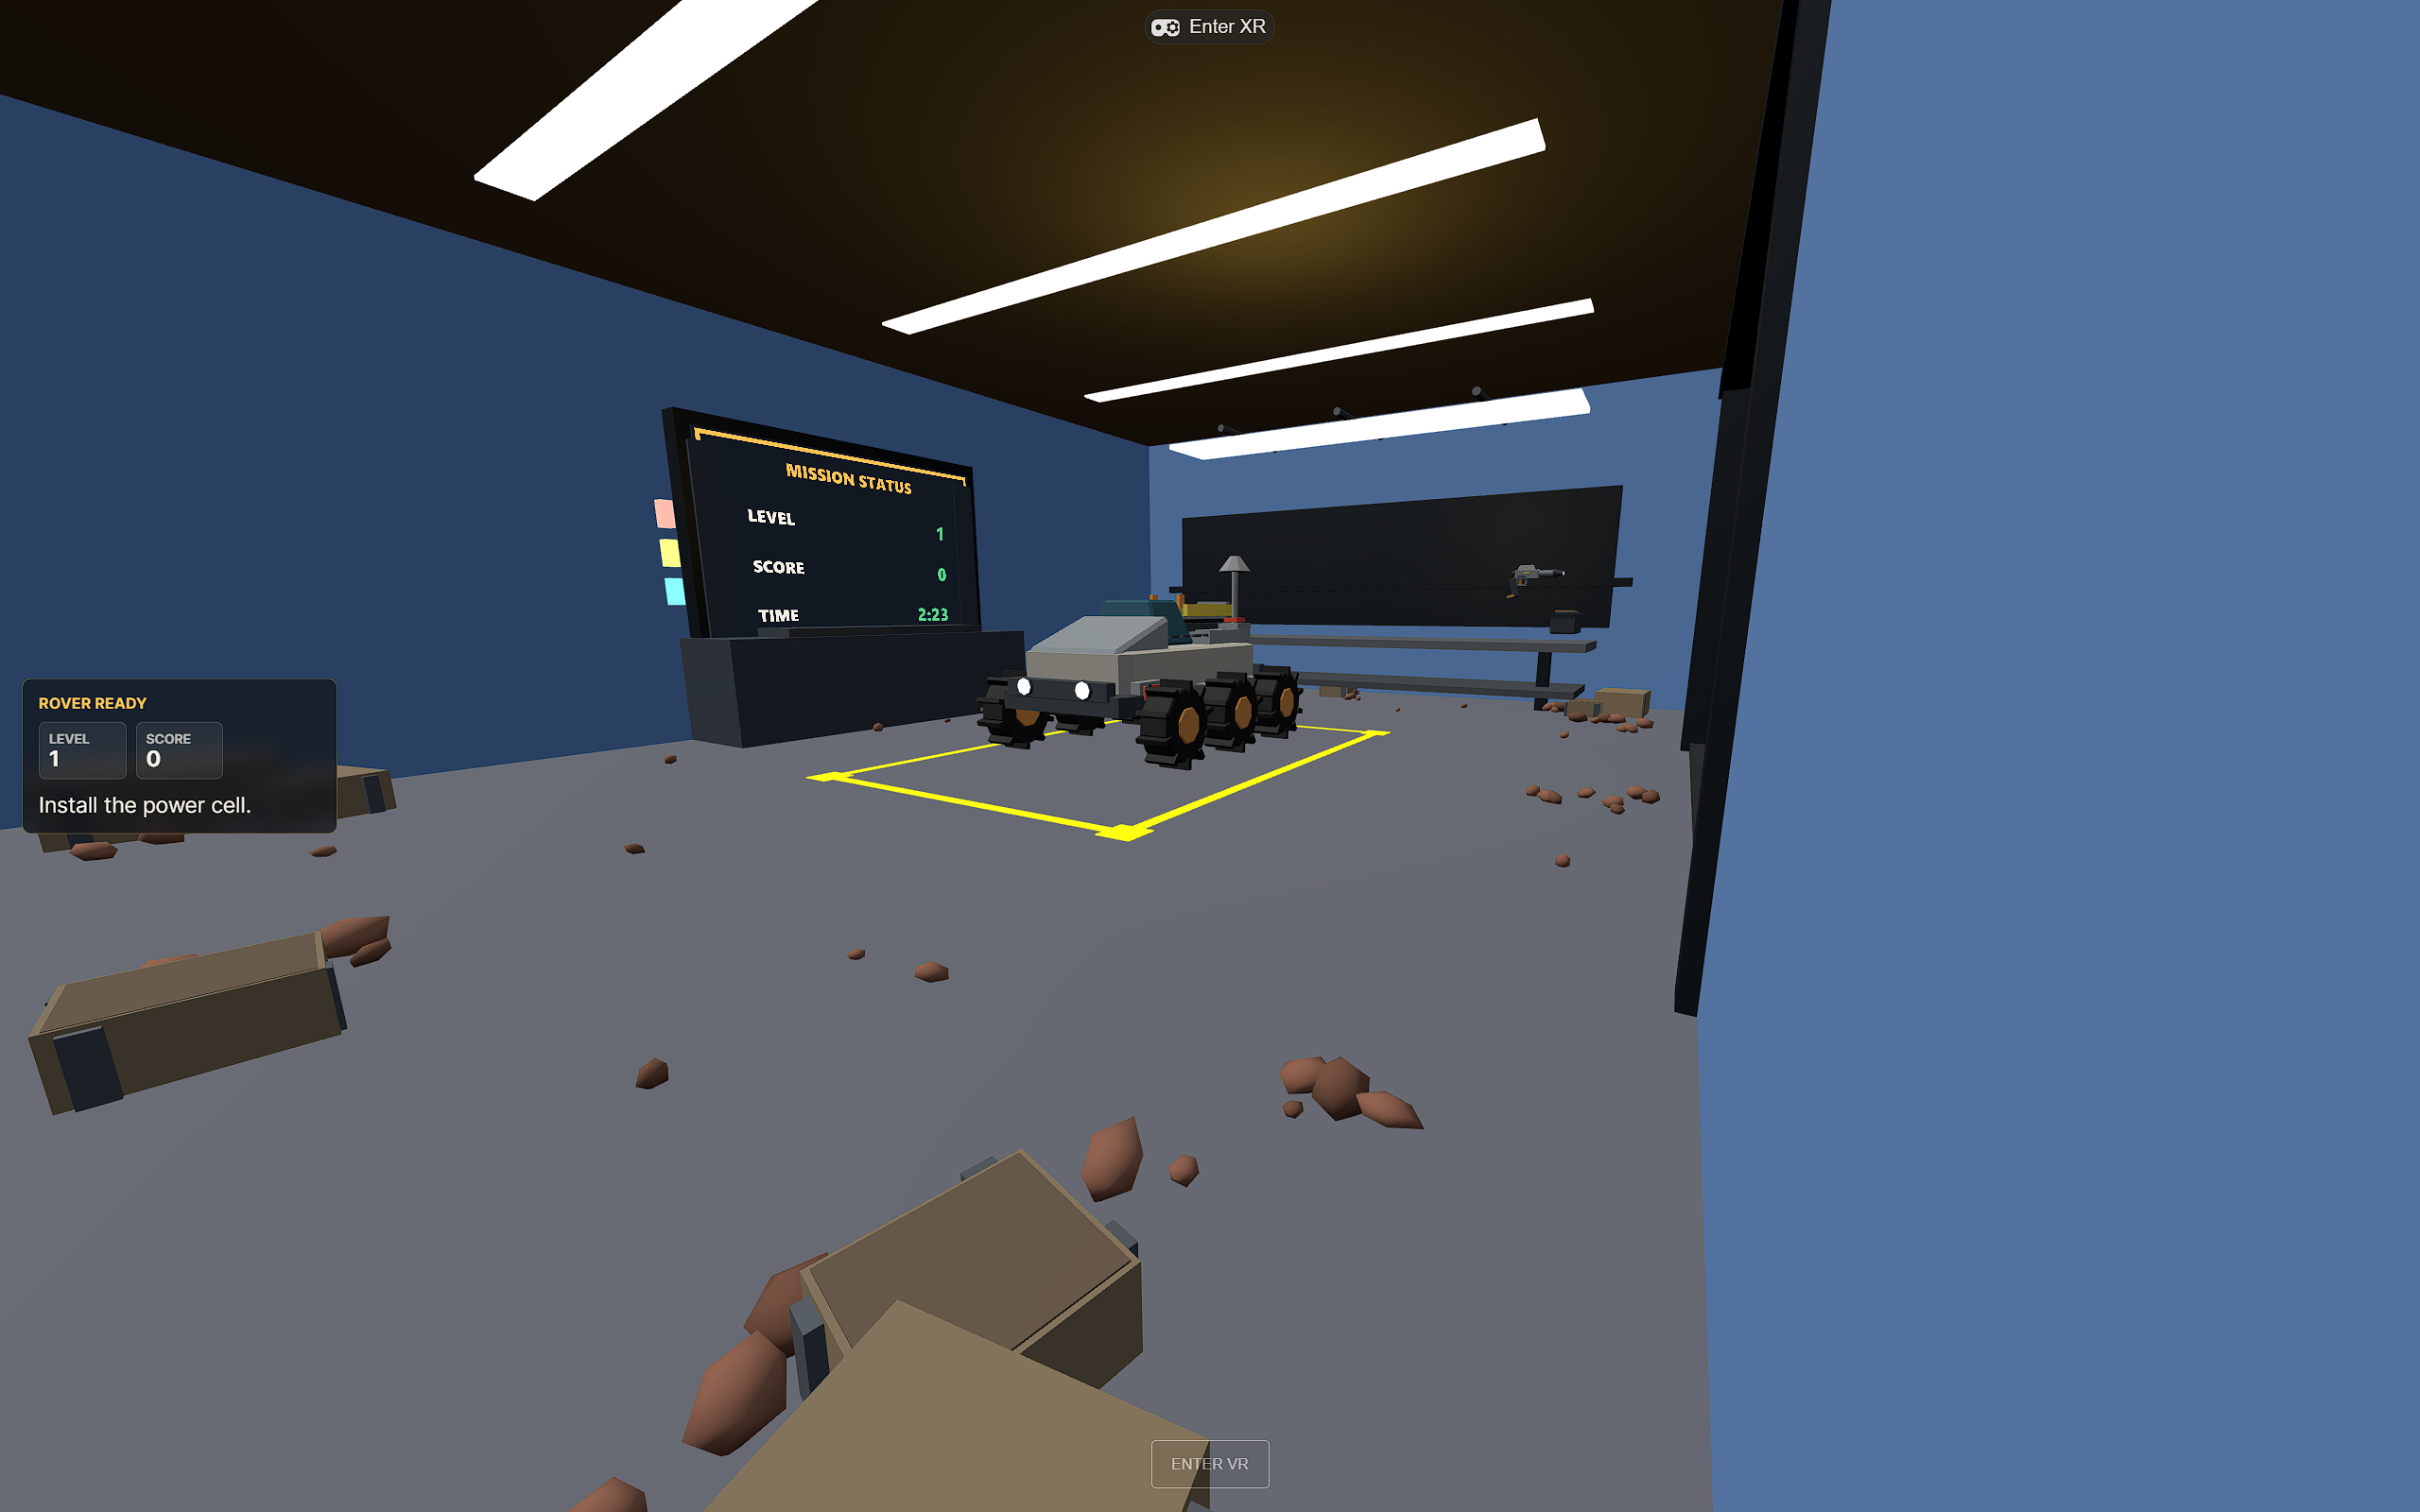
\includegraphics[width=0.32\textwidth]{setup.png}
	\hfill
	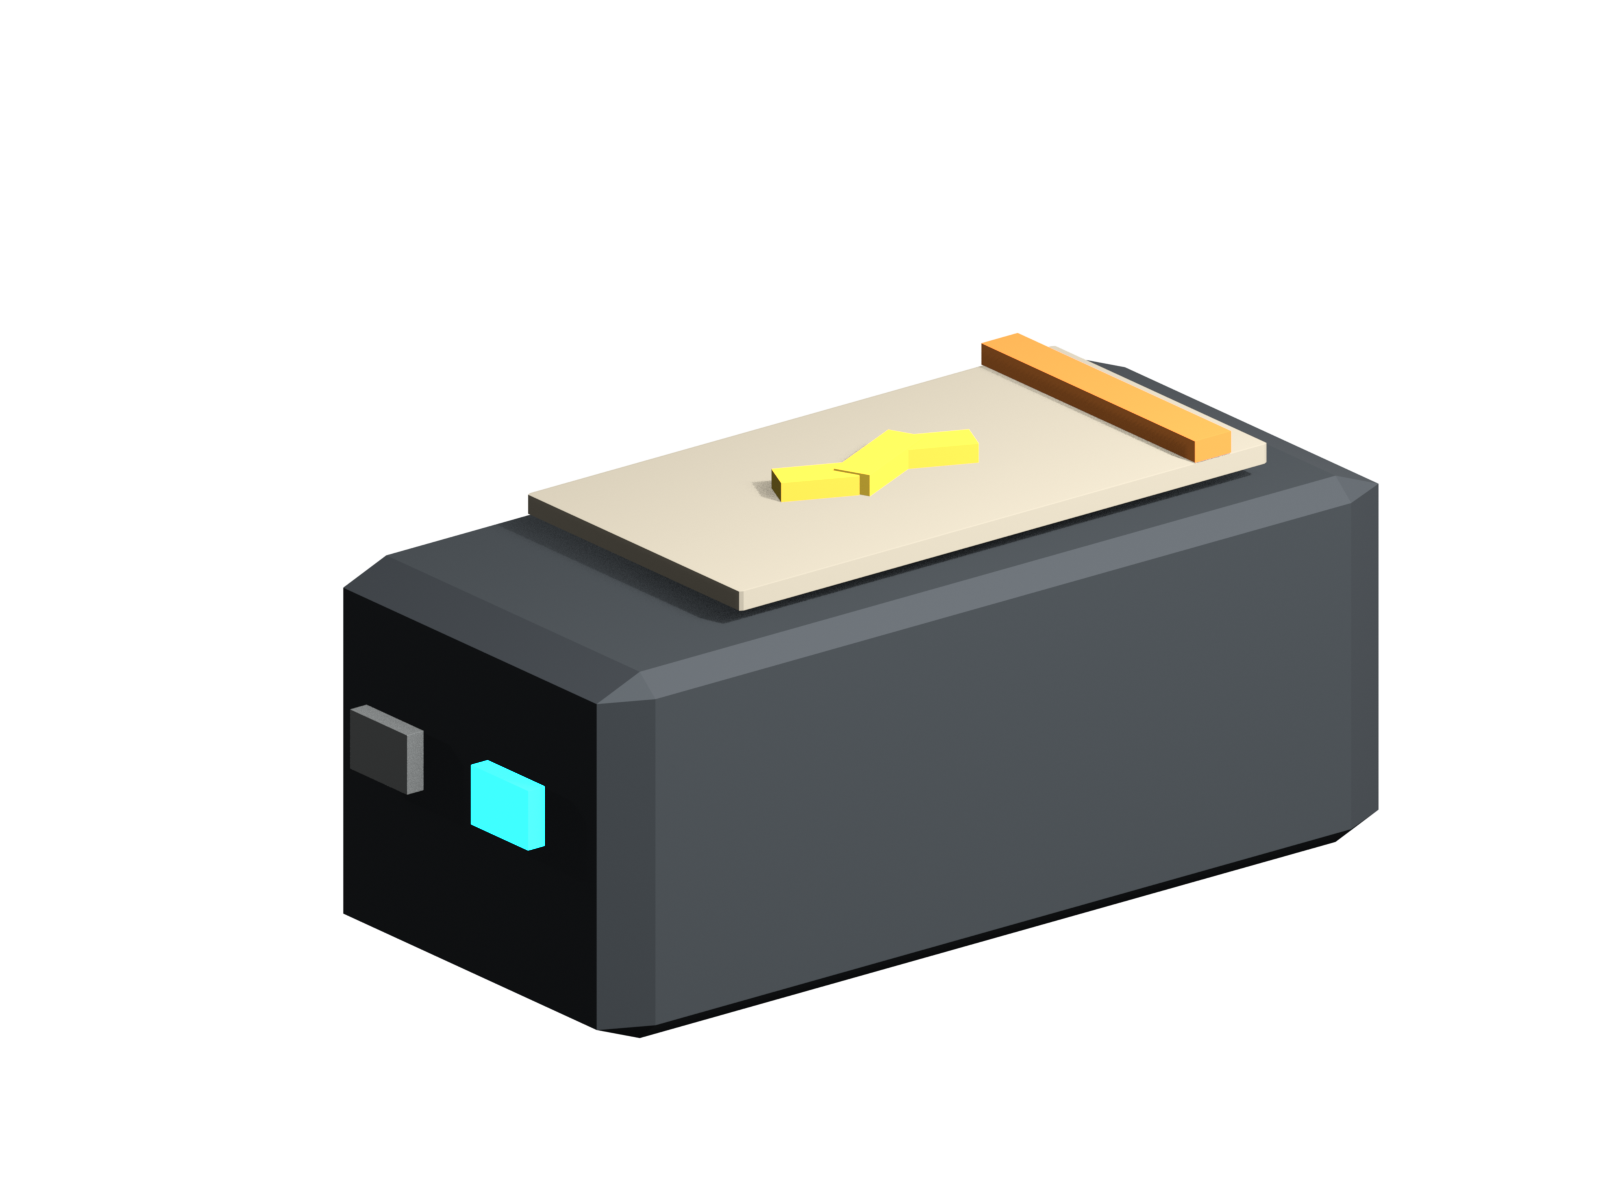
\includegraphics[width=0.32\textwidth]{power_module.png}
	\hfill
	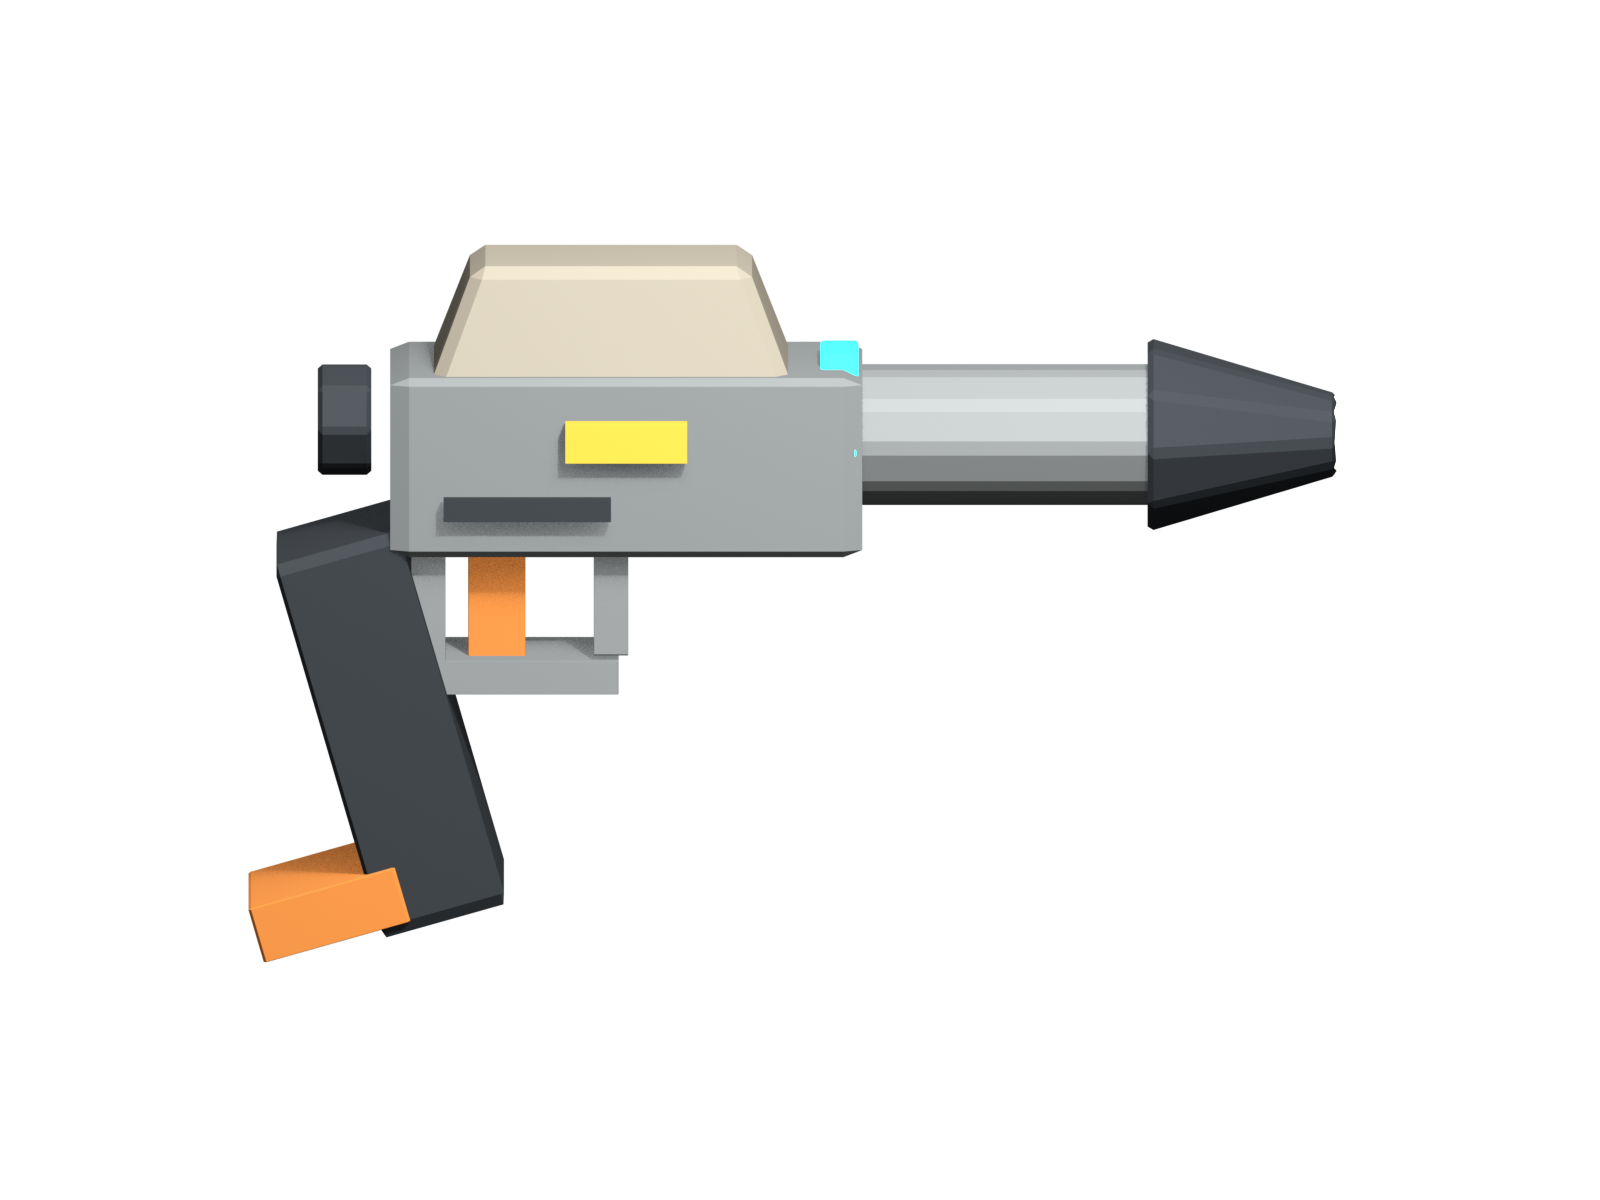
\includegraphics[width=0.32\textwidth]{repair_tool.png}
	\caption{Final demo visuals. Left: the rover parked inside the repair bay.
		Center: the custom power-cell module. Right: the custom handheld repair tool.}\label{fig:demo-visuals}
\end{figure*}

\section{Features Table}

Table~\ref{tab:features} maps the assignment requirements to parts of the final
demo. The base requirements are listed separately from the advanced features.

\begin{table*}[t]
	\caption{Requirement Coverage}\label{tab:features}
	\centering
	\footnotesize
	\begin{tabular}{llll}
		\toprule
		\textbf{Req.}      & \textbf{Type} & \textbf{Coverage}             & \textbf{Section} \\
		\midrule
		Original theme     & Base          & Rover service bay             & Overview         \\
		Custom 3D assets   & Base          & Bay, rovers, cell, tool       & Assets           \\
		Core interactions  & Base          & Power, repair, parts, buttons & Scene            \\
		Physics            & Category A    & Grabbable cells, tool, parts  & Challenges       \\
		Object types/modes & Category A    & Buttons, tools, parts, rovers & Scene            \\
		Blender generation & Supporting    & Python-built project assets   & Execution        \\
		\bottomrule
	\end{tabular}
\end{table*}

\section{Challenges and Solutions}

The hardest part was keeping Blender and the browser code in agreement. It was
not enough for a model to look correct in Blender. The runtime also needed to
know where the power cell should snap, where the repair tool should aim, which
mesh belonged to a removable part, and how large the physics body should be. We
handled this by giving gameplay nodes stable names in the Blender exports, such
as \texttt{RR\_PowerCell\_InsertPoint} and component \texttt{\_SnapTarget}
nodes, then reading those names from JavaScript.

Physics needed a similar compromise. The visible rover and bay meshes are too
detailed to use directly as collision geometry. When we tried to treat visual
shape and gameplay shape as the same thing, small objects became harder to grab
and place. The final version uses simpler Cannon-ES boxes for the table,
power-cell body, repair tool, and loose parts. The GLB meshes still provide the
visual detail, while the physics shapes keep the interaction predictable.

The rover flow also needed more state control than expected. Calling, parking,
checking, opening the door, and sending the rover all touch the same model and
the same collision bodies. The final code separates arrival, turning, repair,
departure turning, and departure movement so the rover does not fight its static
bodies or leave before the door sequence is ready.

Scope was the last major issue. A larger Mars base would have made the project
look bigger but would not have improved the required interactions. We kept the
player in one bay and spent the extra time on snap targets, repair feedback,
button states, and the later complex-rover levels.

\section{Discussion and Future Work}

The best part of the final demo is that the loop is easy to understand without
needing a separate tutorial. The rover stops in a consistent place, the loose
parts spawn on the table, and the buttons control obvious bay actions. The snap
system also helps with usability. The player still has to move the object to the
right area, but the final alignment does not require unrealistic hand precision.

The roughest part is still feedback polish. The HUD, glowing targets, snapped
objects, and button lights communicate the state of the rover, but the repair
tool would feel better with sound, haptics, and a more active animation. The
diagnostic screen could also do more than show status text. It could highlight a
diagram of the rover and point to the next damaged part.

If we continued the project, we would add those feedback pieces before adding a
new room. More repair job types would also fit, but they should stay inside the
same bay structure. The project works best when the player is focused on the
rover instead of searching through a larger environment.

\section{Individual Contributions}

Table~\ref{tab:contributions} lists the main ownership split. The percentages
are approximate and describe who led each area rather than exact time spent.

\begin{table}[b]
	\caption{Individual Contribution Summary}\label{tab:contributions}
	\centering
	\footnotesize
	\begin{tabular}{lll}
		\toprule
		\textbf{Component}      & \textbf{Lead}   & \textbf{Approx. Share} \\
		\midrule
		Asset visual direction  & Chirag Baviskar & 60\% / 40\%            \\
		Asset export/package    & Chirag Baviskar & 70\% / 30\%            \\
		Three.js/WebXR runtime  & Dhrumil Patel   & 30\% / 70\%            \\
		Input handling          & Dhrumil Patel   & 30\% / 70\%            \\
		Physics and collisions  & Dhrumil Patel   & 30\% / 70\%            \\
		Game flow and HUD       & Dhrumil Patel   & 35\% / 65\%            \\
		Final docs/presentation & Chirag Baviskar & 60\% / 40\%            \\
		\bottomrule
	\end{tabular}
\end{table}

\section{Asset Credits}

The garage bay, regular rover, complex rover, power-cell module, repair tool,
and Mars exterior were made for this project in Blender. The source submission
includes the original \path{.blend} files, exported \path{.glb} runtime files,
and the Blender Python scripts used to generate the assets.

The runtime depends on Three.js for rendering and WebXR support, GLTFLoader for
model loading, and Cannon-ES for physics. These are software libraries, not
third-party scene assets. The final visible scene does not use outside 3D
models, outside texture packs, 360-degree media, or Gaussian splats.

\section{Code and Execution Instructions}

After extracting the source zip, use the extracted folder as the project root.
All paths in these instructions are relative to that folder. The runnable
entrypoint is \path{./index.html}. The demo needs a local web server because it
uses JavaScript modules, CDN imports, and GLB asset loading. Opening
\path{./index.html} directly from the file system will not load the demo
correctly.

From the extracted source folder, run one of the included scripts:

\begin{verbatim}
.\run-demo.ps1
run-demo.bat
./run-demo.sh
\end{verbatim}

Each script serves the project at:

\begin{verbatim}
http://localhost:5173/
\end{verbatim}

The same server can be started manually from that folder:

\begin{verbatim}
python -m http.server 5173
\end{verbatim}

Then open \url{http://localhost:5173/} in a Chromium-based browser. Desktop
controls are included for testing: \texttt{W}, \texttt{A}, \texttt{S}, and
\texttt{D} move the player, the arrow keys turn, and mouse dragging grabs
objects. In VR, the controller thumbsticks handle movement and trigger/select
grabs objects. The WebXR Emulator browser extension can be used when a headset
is not available.

The source materials include \path{./index.html}, the JavaScript files under
\path{./src}, runtime GLB files under \path{./src/assets/models}, Blender source
files under \path{./src/assets/blend}, and Blender generation scripts under
\path{./scripts/blender}.

\nocite{three,webxr,cannon,blender}
\bibliographystyle{IEEEtran}
\bibliography{refs}

\end{document}
